\documentclass[a4paper, 12pt]{article}

\input{/home/nick/latex-preambles/xelatex.tex}

\setmainfont{Minion Pro}

\newcommand{\imagesPath}{.}

\title{
	\textbf{Εργαστήριο Δικτύων Υπολογιστών} \\~\\
	Εργαστηριακή Άσκηση 1 \\ 
	Εξοικείωση με το FreeBSD και το VirtualBox
}
\author{}
\date{}

\begin{document}
	\maketitle
	\begin{center}
	\begin{tabular}{|l|l|}
		\hline
		\textbf{Ονοματεπώνυμο:} Νικόλαος Παγώνας, el18175  & \textbf{Όνομα PC:} nick-ubuntu \\
		\hline
		\textbf{Ομάδα:} 1 (Τρίτη 10:45) & \textbf{Ημερομηνία Εξέτασης:} Τρίτη 08/03/2022 \\
		\hline
	\end{tabular}
	\end{center}

\section*{Άσκηση 1: Γνωριμία με το περιβάλλον εργασίας}
	\subsection*{1.1}
		Η διεύθυνση IPv4 του εικονικού VirtualBox Host-Only Ethernet Adapter είναι \verb|192.168.56.1|.
		
	\subsection*{1.2}
		Η μάσκα του τοπικού δικτύου είναι \verb|255.255.255.0|.
	
	\subsection*{1.3}
		Ναι, ο εξυπηρετητής DHCP είναι ενεργοποιημένος.
	
	\subsection*{1.4}
		Η διεύθυνση IPv4 του εξυπηρετητή DHCP είναι \verb|192.168.56.100| και η περιοχή διευθύνσεων που έχει διατεθεί για δυναμική παραχώρηση είναι \verb|192.168.56.101-192.168.56.254|
		
	\subsection*{1.5}
		Το prompt που εμφανίζεται για τον χρήστη \verb|lab| είναι:
		
		\begin{verbatim}
			lab@pc:~%
		\end{verbatim}
	
	\subsection*{1.6}
		Το αποτέλεσμα της εντολής \verb|man| είναι:
		
		\begin{figure}[H]
			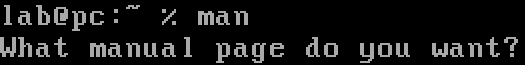
\includegraphics[width=.5\linewidth]{\imagesPath/1.6.png}
		\end{figure}
		
		Αυτό συμβαίνει επειδή δεν έχουμε δώσει ως όρισμα στην \verb|man| μια εντολή για να εμφανιστεί το κατάλληλο manpage.
	
	\subsection*{1.7}
		Το αποτέλεσμα της εντολής \verb|man man| είναι το manual page της ίδιας της εντολής \verb|man|, όπως φαίνεται στην εικόνα.
	
		\begin{figure}[H]
			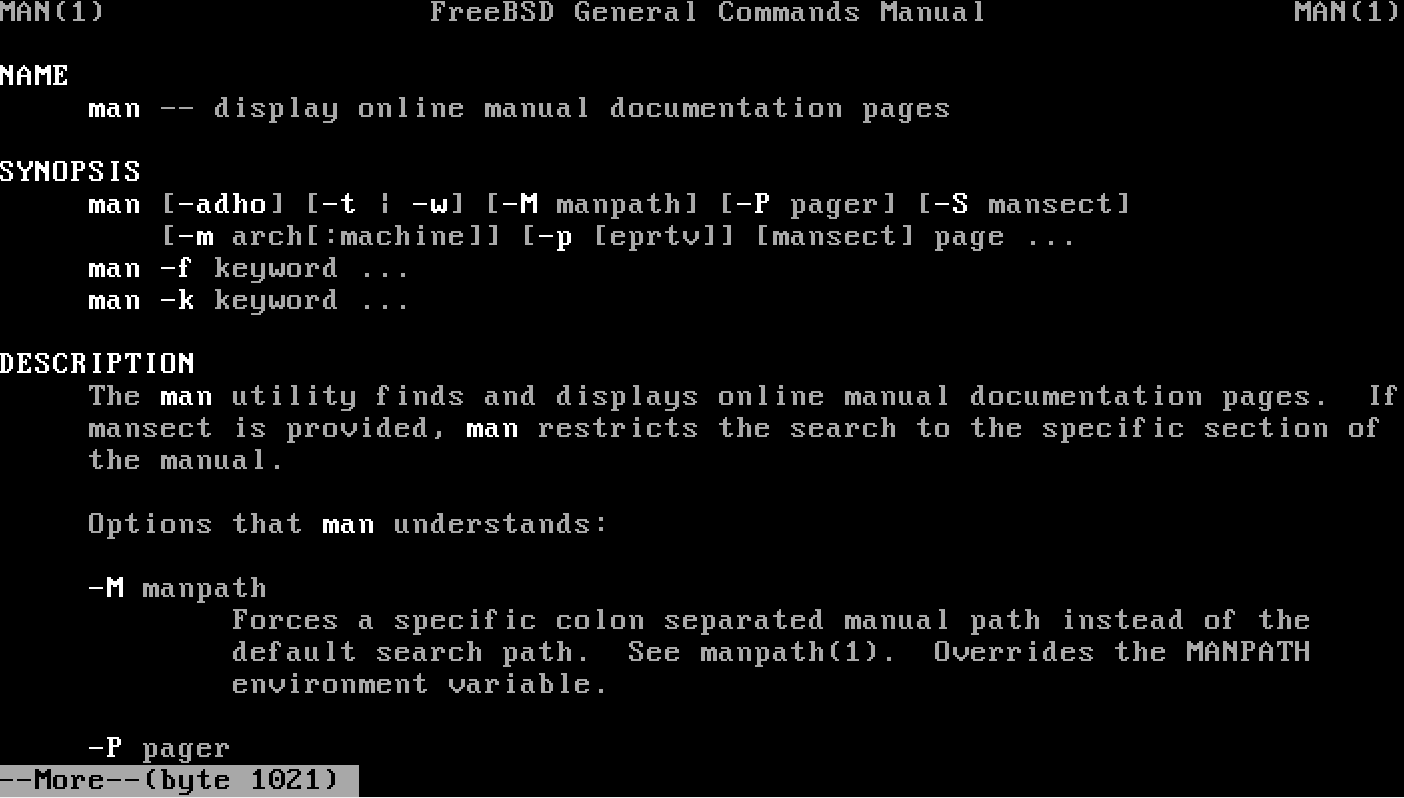
\includegraphics[width=\linewidth]{\imagesPath/1.7.png}
		\end{figure}
	
	\subsection*{1.8}
		Η εντολή \verb|man hier| (\textbf{hier}archy) μας εμφανίζει πληροφορίες για το layout του συστήματος αρχείων μας, όπως φαίνεται και στην εικόνα.
	
		\begin{figure}[H]
			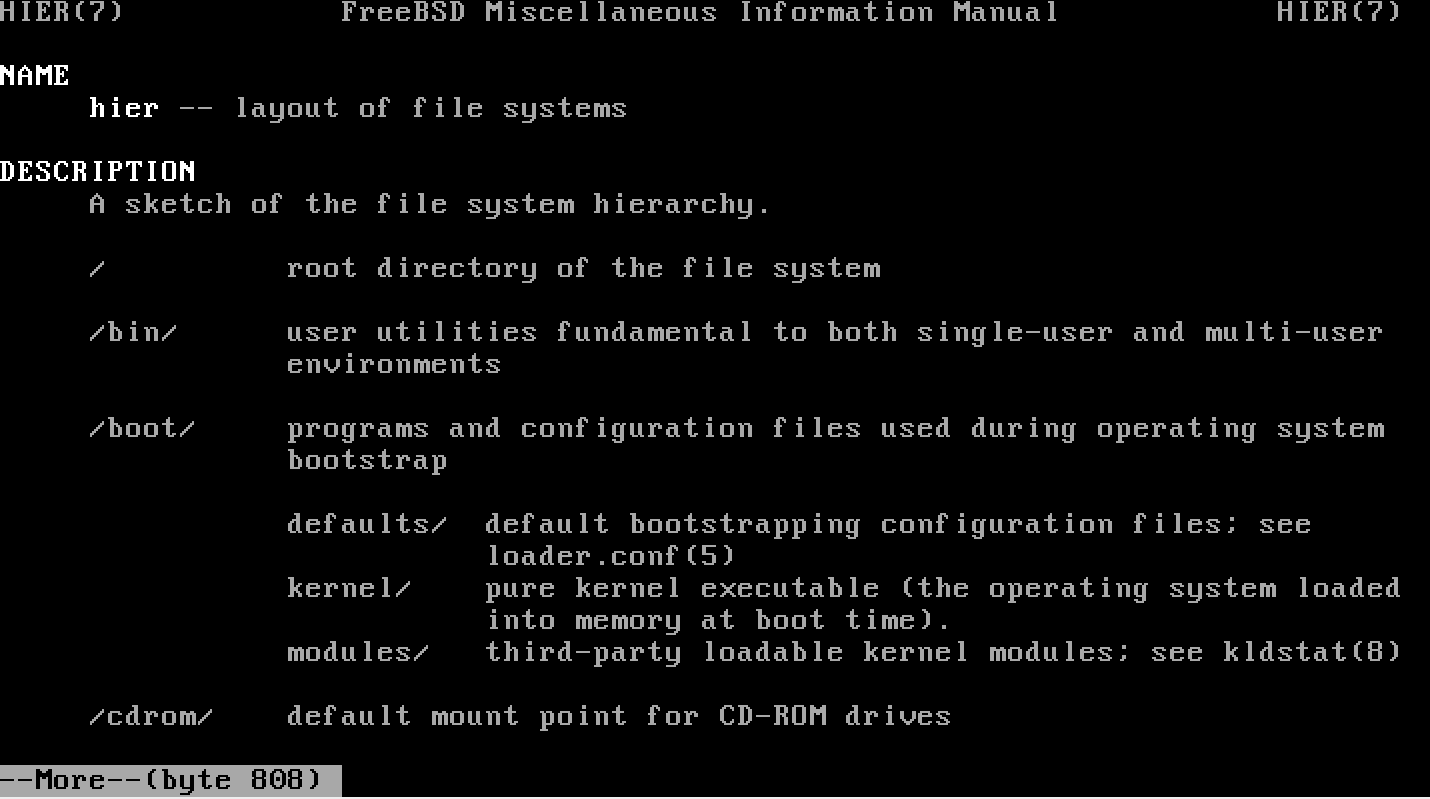
\includegraphics[width=\linewidth]{\imagesPath/1.8.png}
		\end{figure}
	
	\subsection*{1.9}
		Σύμφωνα με το αποτέλεσμα της προηγούμενης εντολής, ο κατάλογος \verb|/lib| περιέχει τις κρίσιμες βιβλιοθήκες που χρειάζονται για τα εκτελέσιμα στους καταλόγους \verb|/bin| και \verb|/sbin|.
			
	\subsection*{1.10}
		Οι θυρίδες ηλεκτρονικού ταχυδρομείου των χρηστών βρίσκονται στον κατάλογο \verb|/var/mail|.
	
	\subsection*{1.11}
		Μπορούμε να μετακινηθούμε με τα πλήκτρα: 
		
		\begin{itemize}
			\item Πάνω/κάτω βελάκι για μία γραμμή πάνω/κάτω αντίστοιχα
			\item \verb|J/K| για μια γραμμή κάτω/πάνω αντίστοιχα
			\item \verb|Space| για να κατέβουμε μία σελίδα κάτω
			\item \verb|PgUp/PgDn| για να ανέβουμε/κατέβουμε μία σελίδα πάνω/κάτω αντίστοιχα.
		\end{itemize}
		
		Γενικά υπάρχουν πολλοί τρόποι. Άλλα πλήκτρα που μπορούμε να χρησιμοποιήσουμε για να μετακινηθούμε είναι \verb|ENTER, e, d, b, w, y, u, f| και πολλά άλλα, καθώς και συνδυασμοί ορισμένων από αυτά με \verb|CTRL| και \verb|ESC|.
	
	\subsection*{1.12}
		Για να αναζητήσουμε μια συγκεκριμένη λέξη-pattern, πατάμε \verb|/| ακολουθούμενο από την λέξη που επιθυμούμε, δηλαδή \verb|/pattern| και πατάμε \verb|ENTER|. Μετά με \verb|N| βρίσκουμε την επόμενη εμφάνιση της λέξης.
			
	\subsection*{1.13}
		Το βασικό πλεονέκτημα της \verb|less| σε σχέση με την \verb|more| είναι ότι με την \verb|less| μπορούμε να πάμε και πίσω στο αρχείο, όχι μόνο μπροστά.
	
	\subsection*{1.14}
		Με την εντολή \verb|hostname| βρίσκουμε ότι το όνομα του εικονικού μηχανήματος είναι \verb|pc.ntua.lab|.
	
	\subsection*{1.15}
		Με την εντολή \verb|whoami| επιβεβαιώνουμε ότι το όνομα χρήστη με το οποίο έχουμε συνδεθεί είναι \verb|lab|.
	
	\subsection*{1.16}
	 	Με την εντολή \verb|id| βρίσκουμε ότι ο αριθμός ταυτότητας του χρήστη \verb|lab| είναι \verb|1001|.
	
	\subsection*{1.17}
		Πάλι από την εντολή \verb|id| βλέπουμε ότι ο χρήστης \verb|lab| ανήκει στις ομάδες \verb|lab| και \verb|wheel|.
	
	\subsection*{1.18}
		Κάνουμε \verb|cd ~| για να πάμε στον \verb|home| φάκελο του χρήστη \verb|lab|. Ύστερα γράφουμε \verb|pwd| και βλέπουμε ότι ο φάκελος αυτός είναι ο \verb|/usr/home/lab|.
	
	\subsection*{1.19}
		To prompt που εμφανίζεται για τον διαχειριστή \verb|root| είναι:
		
		\begin{verbatim}
			root@pc:~#
		\end{verbatim}
	
	\subsection*{1.20}
		O αριθμός ταυτότητας του \verb|root| είναι 0 (εντολή \verb|id|).
	
	\subsection*{1.21}
		Ο διαχειριστής ανήκει στις ομάδες χρηστών \verb|wheel| και \verb|operator| (εντολή \verb|id|).
	
	\subsection*{1.22}
		Ο αριθμός ταυτότητας (gid) της ομάδας \verb|wheel| είναι \verb|0|.
	
	\subsection*{1.23}
		Ο \verb|home| φάκελος εργασίας του \verb|root| είναι ο \verb|/root|. (εντολή \verb|pwd|).
	
	\subsection*{1.24}
		Η διεύθυνση που αποδόθηκε στο εικονικό μας μηχάνημα από τον εξυπηρετητή DHCP είναι η \verb|192.168.56.101|.
	
	\subsection*{1.25}
		Με την εντολή \verb|ifconfig| βρίσκουμε ότι το μηχάνημα διαθέτει τις διεπαφές \verb|em0| και \verb|lo0|.
	
	\subsection*{1.26}
		Πάλι μέσω της εντολής \verb|ifconfig| (πεδίο \verb|ether|) βρίσκουμε ότι η διεύθυνση MAC της κάρτας δικτύου \verb|em0| του εικονικού μηχανήματος είναι \verb|08:00:27:e8:17:4a|.
	
	\subsection*{1.27}
		Πάλι μέσω της εντολής \verb|ifconfig| βρίσκουμε ότι η ταχύτητα της κάρτας δικτύου \verb|em0| είναι \verb|1 Gbps|.
	
	\subsection*{1.28}
		Πάλι μέσω της εντολής \verb|ifconfig| (πεδίο \verb|inet|) βλέπουμε ότι η διεύθυνση IPv4 της διεπαφής που αντιστοιχεί στην κάρτα δικτύου \verb|em0| είναι \verb|192.168.56.101|.
	
	\subsection*{1.29}
		Πάλι μέσω της εντολής \verb|ifconfig| (πεδίο \verb|netmask|), βρίσκουμε ότι η μάσκα υποδικτύου σε hex μορφή είναι \verb|0xffffff00|, δηλαδή \verb|255.255.255.0| σε δεκαδική μορφή.  
	
	\subsection*{1.30}
		Πάλι μέσω της εντολής \verb|ifconfig| (πεδίο \verb|mtu|), βρίσκουμε ότι η MTU είναι 1500 (bytes). 
	
	\subsection*{1.31}
		\verb|lo0:|
		\begin{itemize}
			\item Διεύθυνση IPv4: \verb|127.0.0.1|
			\item Μάσκα υποδικτύου: \verb|255.0.0.0|
			\item MTU: 16384 (bytes)
		\end{itemize}
	
	\subsection*{1.32}
		Εκτελώντας \verb|cat /etc/resolv.conf| παίρνουμε κενή έξοδο (το αρχείο δεν περιέχει τίποτα), άρα δεν έχουν οριστεί εξυπηρετητές DNS.

	\subsection*{1.33}
		Αν κάνουμε από το φιλοξενούμενο μηχάνημα \verb|ping 192.168.56.1|, τότε το φιλοξενούν μηχάνημα απαντάει.
	
	\subsection*{1.34}
		Αν κάνουμε από το φιλοξενούν μηχάνημα \verb|ping 192.168.56.101|, τότε το φιλοξενούμενο μηχάνημα απαντάει.
	
	\subsection*{1.35}
		Η εντολή \verb|ping| στέλνει για πάντα πακέτα, μέχρι να την διακόψουμε, ενώ η αντίστοιχη των Windows στέλνει μόνο 4 by default.

\section*{Άσκηση 2: Βασικές εντολές συστήματος αρχείων}

	\subsection*{2.1}
		Με την εντολή \verb|pwd| βρίσκουμε ότι το home directory για τον χρήστη \verb|lab| είναι \verb|/usr/home/lab|.

	\subsection*{2.2}
		Mε την εντολή \verb|mkdir tmp| δημιουργούμε έναν νέο φάκελο \verb|tmp|.

	\subsection*{2.3}
		Με την εντολή \verb|mkdir tmp/el18175| δημιουργούμε έναν νέο φάκελο \verb|el18175| κάτω από το \verb|tmp|.

	\subsection*{2.4}
		Με την εντολή \verb|cd tmp/el18175| μετακινούμαστε στον φάκελο \verb|el18175|.

	\subsection*{2.5}
		Με την εντολή \verb|find / -name hosts| βρίσκουμε ότι αρχείο με όνομα \verb|hosts| βρίσκεται στις τοποθεσίες \verb|/usr/share/examples/etc/hosts|, \verb|/etc/bluetooth/hosts| και \verb|/etc/hosts|.

	\subsection*{2.6}
		Με την εντολή \verb|cp /etc/hosts ~/tmp/el18175| αντιγράφουμε το αρχείο \verb|/etc/hosts| στον φάκελο \verb|~/tmp/el18175| που δημιουργήσαμε.

	\subsection*{2.7}
		Με την εντολή \verb|mv hosts hostsfile| αλλάζουμε το όνομα του αρχείου \verb|hosts| σε \verb|hostsfile|.

	\subsection*{2.8}
		Mε την εντολή \verb|ls -l| βλέπουμε ότι το hostsfile έχει τα permission flags \verb|-rw-r--r--|. Το πρώτο \verb|r| σημαίνει ότι ο ιδιοκτήτης του αρχείου (user) έχει δικαίωμα ανάγνωσης στο συγκεκριμένο αρχείο, το \verb|w| σημαίνει ότι ο ιδιοκτήτης του αρχείου έχει δικαίωμα εγγραφής, το δεύτερο \verb|r| σημαίνει ότι οι χρήστες που ανήκουν στην ίδια ομάδα χρηστών (group) με τον ιδιοκτήτη έχουν δικαίωμα ανάγνωσης, και το τρίτο \verb|r| σημαίνει ότι οι υπόλοιποι χρήστες (others) έχουν δικαίωμα ανάγνωσης. 

	\subsection*{2.9}
		Με την εντολή \verb|touch test| δημιουργούμε ένα νέο άδειο αρχείο με όνομα \verb|test|.

	\subsection*{2.10}
		Με την εντολή \verb|touch .hidden| δημιουργούμε ένα νέο κρυφό άδειο αρχείο με όνομα \verb|.hidden| (είναι κρυφό λόγω της τελείας που βρίσκεται στην αρχή).

	\subsection*{2.11}
		Με την εντολή \verb|ls -l /etc/services| βρίσκουμε ότι το αρχείο \verb|/etc/services| έχει μέγεθος 86674 (bytes).

	\subsection*{2.12}
		Γενικά, η εντολή \verb|df| εμφανίζει στατιστικά σχετικά με τον ελεύθερο χώρο της συσκευής. Η διαφορά των \verb|df -H| και \verb|df -h| είναι ότι η πρώτη εμφανίζει τα μεγέθη σε δυνάμεις του 1024, ενώ η δεύτερη σε δυνάμεις του 1000.

	\subsection*{2.13}
		Με την εντολή \verb|df -h ./| (βρισκόμαστε στον φάκελο \verb|el18175|) βλέπουμε ότι έχουμε \verb|6.5 Gigabyte| ελεύθερο χώρο, που είναι παραπάνω από αρκετός.

	\subsection*{2.14}
		Με την εντολή \verb|cp /etc/services ./| αντιγράφουμε το αρχείο \verb|/etc/services| στον φάκελό μας.

	\subsection*{2.15}
		Με την εντολή \verb|gzip services| συμπιέζουμε το αρχείο \verb|services|, και με την εντολή \verb|ls -l| βρίσκουμε ότι το νέο μέγεθός του είναι \verb|24577 bytes|.

	\subsection*{2.16}
		Με την εντολή \verb|ls -a| βλέπουμε τα περιεχόμενα του φακέλου μας συμπεριλαμβανομένων και των κρυφών αρχείων.

	\subsection*{2.17}
		Με την εντολή \verb|find /usr -user lab| βρίσκουμε όλα τα αρχεία του καταλόγου \verb|/usr| που ανήκουν στον χρήστη \verb|lab|. Είναι τα εξής:
		
		\begin{verbatim}
			/usr/home/lab
			/usr/home/lab/.login
			/usr/home/lab/.rhosts
			/usr/home/lab/.mail_aliases
			/usr/home/lab/.profile
			/usr/home/lab/.cshrc
			/usr/home/lab/.login_conf
			/usr/home/lab/.shrc
			/usr/home/lab/.mailrc
			/usr/home/lab/.history
			/usr/home/lab/.lesshst
			/usr/home/lab/tmp
			/usr/home/lab/tmp/el18175
			/usr/home/lab/tmp/el18175/test
			/usr/home/lab/tmp/el18175/hostsfile
			/usr/home/lab/tmp/el18175/services.gz
		\end{verbatim}

	\subsection*{2.18}
		Με την εντολή \verb|rm ~/tmp/el18175/*| διαγράφουμε όλα τα αρχεία που περιέχει ο φάκελος με όνομα τον αριθμό μητρώου μας. 

	\subsection*{2.19}
		Με την εντολή \verb|rm -r ~/tmp| διαγράφουμε τον φάκελο \verb|tmp| που δημιουργήσαμε και ό,τι αυτός περιέχει.

\section*{Άσκηση 3: Επεξεργασία κειμένου, ανακατεύθυνση εντολών}

	\subsection*{3.1}
		Οι εντολές του \verb|vi| που χρησιμοποιήσαμε είναι:
			\begin{itemize}
				\item \verb|:%s /localhost/ntua-lab/g|
				\item \verb|:q!|
			\end{itemize}
			
	\subsection*{3.2}
		Με την εντολή \verb|ls -l /etc > filelist| δημιουργούμε ένα νέο αρχείο με όνομα \verb|filelist| που περιέχει την έξοδο της εντολής \verb|ls -l /etc|.

	\subsection*{3.3}
		Με την εντολή \verb|vi filelist| ανοίγουμε το αρχείο στον \verb|vi| για επεξεργασία. Μέσα στον \verb|vi|, εκτελούμε \verb|dd| για να διαγράψουμε την πρώτη γραμμή του αρχείου, και ύστερα εκτελούμε \verb|:wq| για να αποθηκεύσουμε τις αλλαγές και να επιστρέψουμε στην γραμμή εντολών. Ο \verb|vi| μας ενημερώνει ότι το νέο αρχείο έχει \verb|101| γραμμές και \verb|5949| χαρακτήρες.

	\subsection*{3.4}
		Η γραμμή που σβήσαμε δείχνει πόσo χώρο (μετρημένο σε filesystem blocks) πιάνουν τα αρχεία του φακέλου στον οποίο εκτελέσαμε \verb|ls -l|.

	\subsection*{3.5}
		Μπορούμε να εκτελέσουμε την εντολή \verb|wc filelist|, η οποία μας επιστρέφει ότι το αρχείο \verb|filelist| περιέχει \verb|101| γραμμές, \verb|917| λέξεις, και \verb|5949| χαρακτήρες.

	\subsection*{3.6}
		Μπορούμε να εκτελέσουμε \verb+ls -l /etc | wc+, που θα μας επιστρέψει \verb|102| γραμμές, οπότε αν αφαιρέσουμε μία γραμμή (λόγω του \verb|total ...|) βρίσκουμε το ίδιο αποτέλεσμα με πριν.
	
	\subsection*{3.7}
		Με την εντολή \verb+ls -l /etc | grep "rc" | wc+ βρίσκουμε ότι \verb|14| αρχεία του καταλόγου \verb|/etc| περιέχουν το κείμενο \verb|"rc"| στο όνομά τους.

\section*{Άσκηση 4: Βασικές πληροφορίες συστήματος}

	\subsection*{4.1}
		Με την εντολή \verb+grep -i cpu /var/run/dmesg.boot+ παίρνουμε τις εξής πληροφορίες για τον επεξεργαστή: 
		
		\begin{verbatim}
			CPU: Intel(R) Core(TM) i7-8565U CPU @ 1.80GHz (1991.76-MHz 686-class CPU)
		\end{verbatim}

	\subsection*{4.2}
		Με την εντολή \verb+grep -i memory /var/run/dmesg.boot+ παίρνουμε τις εξής πληροφορίες για την μνήμη:
		
		\begin{verbatim}
			real memory  = 268369920 (255 MB)
			avail memory = 239337472 (228 MB)
		\end{verbatim}

	\subsection*{4.3}
		Με την εντολή \verb|uname -v| παίρνουμε τις εξής πληροφορίες για τη έκδοση του λειτουργικού συστήματος:
		
		\begin{verbatim}
			FreeBSD 10.0-RELEASE #0 r260789: Fri Jan 17 01:46:25 UTC 2014     
			root@snap.freebsd.org:/usr/obj/usr/src/sys/GENERIC 
		\end{verbatim}

	\subsection*{4.4}
		 Με την εντολή \verb+service -e | wc+ βρίσκουμε ότι υπάρχουν \verb|16| ενεργοποιημένες υπηρεσίες.

	\subsection*{4.5}
		 Μπορούμε να δούμε τη λίστα όλων των διεργασιών που τρέχουν στο σύστημα με την εντολή \verb|ps -aux|.

	\subsection*{4.6}
		 Με οποιαδήποτε από τις εντολές:
		 
		 \begin{itemize}
		 	\item \verb+ps -aux | grep syslogd+
		 	\item \verb+system -e | grep syslogd+
		 	\item \verb+top | grep syslogd+ 
		 \end{itemize}
		 μπορούμε να δούμε αν τρέχει η υπηρεσία \verb|syslogd|. 

	\subsection*{4.7}
		Με την εντολή \verb|sockstat -4| μπορούμε να βρούμε τις υπηρεσίες που αναμένουν κίνηση \verb|IPv4|, και τις αντίστοιχες θύρες \verb|TCP| ή \verb|UDP| όπου την περιμένουν.

	\subsection*{4.8}
		Με την εντολή \verb|top| βλέπουμε τις πιο κοστοβόρες διεργασίες. Αν θέλουμε να δούμε για κάποια συγκεκριμένη διεργασία, εκτελούμε \verb+top | grep <process name>+.

	\subsection*{4.9}
		Με την εντολή \verb|iostat -d ada0 -w 1| μπορούμε να δούμε τη δραστηριότητα του δίσκου \verb|ada0| ανά δευτερόλεπτο.

	\subsection*{4.10}
		Με την εντολή \verb|vmstat -w 2| μπορούμε να δούμε τη δραστηριότητα της μνήμης (μέση και ελεύθερη) ανά δύο δευτερόλεπτα.

\section*{Άσκηση 5: Πρόσβαση ως root}

	\subsection*{5.1}
		Η πρώτη προσπάθεια απέτυχε, διότι το μηχάνημα δεν επιτρέπει απομακρυσμένη σύνδεση ως \verb|root| για λόγους ασφαλείας.

	\subsection*{5.2}
		Ως χρήστης (lab), δεν μπορούμε να αλλάξουμε το όνομα του εικονικού μηχανήματος σε \verb|virtualmachine|, διότι αυτή η εντολή απαιτεί δικαιώματα διαχειριστή (root). Η εντολή που προσπαθήσαμε να εκτελέσουμε είναι \verb|hostname virtualmachine|.

	\subsection*{5.3}
		O DHCP Server έχει IPv4 διεύθυνση \verb|192.168.56.100|. Εκτελούμε λοιπόν: \\ 
		\verb|ping -c 5 -i 2 192.168.56.100|.

	\subsection*{5.4}
		Η κλήση με διάστημα ενδιάμεσης παύσης \verb|0.1 sec| θα αποτύχει, γιατί το διάστημα είναι πολύ μικρό, μόνο ο διαχειριστής μπορεί να ορίσει τόσο μικρό διάστημα. 

	\subsection*{5.5}
		Για να πετύχουν οι εντολές των ερωτημάτων 5.2 και 5.4, πρέπει να εκτελέσουμε \verb|su| και ύστερα να εισάγουμε τον κωδικό \verb|ntua|. Έτσι θα είμαστε πλέον σε mode διαχειριστή (root) και οι παραπάνω εντολές θα πετύχουν.
		
		Αν θέλουμε να πετυχαίνει \textbf{και} η εντολή του 5.1, θα πρέπει να αλλάξουμε τις ρυθμίσεις \verb|ssh|:
		
		\begin{verbatim}
			vi /etc/ssh/sshd_config
			
			replace: #PermitRootLogin no 
			with: PermitRootLogin yes
			
			/etc/rc.d/sshd restart
		\end{verbatim}
		
		Πλέον μπορούμε να συνδεθούμε και απομακρυσμένα ως root κατευθείαν (χωρίς να χρειάζεται \verb|su|).

	\subsection*{5.6}
		Με τις εντολές \verb|w| ή \verb|who| μπορούμε να δούμε ποιοι χρήστες είναι συνδεδεμένοι στο σύστημα.

	\subsection*{5.7}
		Αν κάποιος κοινός χρήστης λάβει δικαιώματα διαχειριστή, εμφανίζεται στην κονσόλα του εικονικού μηχανήματος προειδοποιητικό μήνυμα. 

	\subsection*{5.8}
		Με την εντολή \verb|cat /var/log/auth.log| βλέπουμε όλα τα μηνύματα σχετικά με authentication/login κλπ. Το μήνυμα που είδαμε πριν στην κονσόλα του εικονικού μηχανήματος εμφανίζεται (μεταξύ άλλων σχετικών μηνυμάτων).

	\subsection*{5.9}
		Με την εντολή \verb|su -l lab| προσομοιώνουμε ένα πλήρες login (με κατάλληλη αλλαγή των μεταβλητών περιβάλλοντος) ως \verb|lab|. Δεν χρειάζεται κωδικός αφού εκτελούμε την εντολή αυτή σε ρόλο διαχειριστή.

\section*{Άσκηση 6: Μεταφορά αρχείων}

	Αρχικά συνδεόμαστε μέσω \verb|sftp| στο εικονικό μηχάνημα με την εντολή \verb|sftp lab@192.168.56.101|.
	Όλες οι παρακάτω εντολές εκτελούνται μέσω \verb|sftp|.
	
	\subsection*{6.1}
		Αντιγράφουμε τα περιεχόμενα του φακέλου \verb|/usr/home/lab| σε φάκελο \verb|~/Downloads/tmp|, με τις εντολές:
		
		\begin{verbatim}
			Initial local directory: ~ (/home/nick)
			Initial remote directory: /usr/home/lab
		
			lcd Downloads (Local directory is now ~/Downloads)
			!mkdir tmp (Directory ~/Downloads/tmp now exists)
			lcd tmp (Local directory is now ~/Downloads/tmp)
			get * (remote: /usr/home/lab/* --> local: ~/Downloads/tmp)
		\end{verbatim}

	\subsection*{6.2}
		Βρισκόμαστε στα ίδια local/remote directories με πριν και εκτελούμε:
		
		\begin{verbatim}
			get /etc/hosts
			get /etc/rc.conf
		\end{verbatim}

	\subsection*{6.3}
		Με την εντολή \verb|mkdir tmp| φτιάχνουμε έναν φάκελο \verb|tmp| κάτω από τον φάκελο του χρήστη \verb|lab|.

	\subsection*{6.4}
		Με την εντολή \verb|put *| αντιγράφουμε τα περιεχόμενα του φακέλου \verb|tmp| του υπολογιστή μας στον φάκελο \verb|tmp| του εικονικού μηχανήματος.

	\subsection*{6.5}
		Με την εντολή \verb|rm *| διαγράφουμε όλα τα περιεχόμενα του φακέλου \verb|tmp| στο εικονικό μηχάνημα.

	\subsection*{6.6}
		Βρισκόμαστε στον φάκελο \verb|/usr/home/lab| και εκτελούμε \verb|rmdir tmp| για να διαγράψουμε τον φάκελο \verb|tmp| από το εικονικό μηχάνημα.

	\subsection*{6.7}
		Με local directory \verb|~/Downloads/tmp| εκτελούμε \verb|get -r /etc/|.

	\subsection*{6.8}
		Η μεταφορά αυτή δεν ολοκληρώνεται γιατί δεν έχουμε δικαίωμα πρόσβασης σε κάποια αρχεία.

	\subsection*{6.9}
		Εκτελούμε \verb|put -r etc|.

	\subsection*{6.10}
		\textbf{Από το τερματικό του εικονικού μηχανήματος} εκτελούμε \verb|mv etc tmp|.

	\subsection*{6.11}
		Ναι, μπορούμε να διαγράψουμε τα περιεχόμενα του φακέλου \verb|tmp|.

	\subsection*{6.12}
		Nαι, μπορούμε να διαγράψουμε τον φάκελο \verb|tmp|.
\end{document}